\chapter{Project planning}


\section{Task breakdown structure}
%Begin from here

\begin{figure}[H]
    \centering
    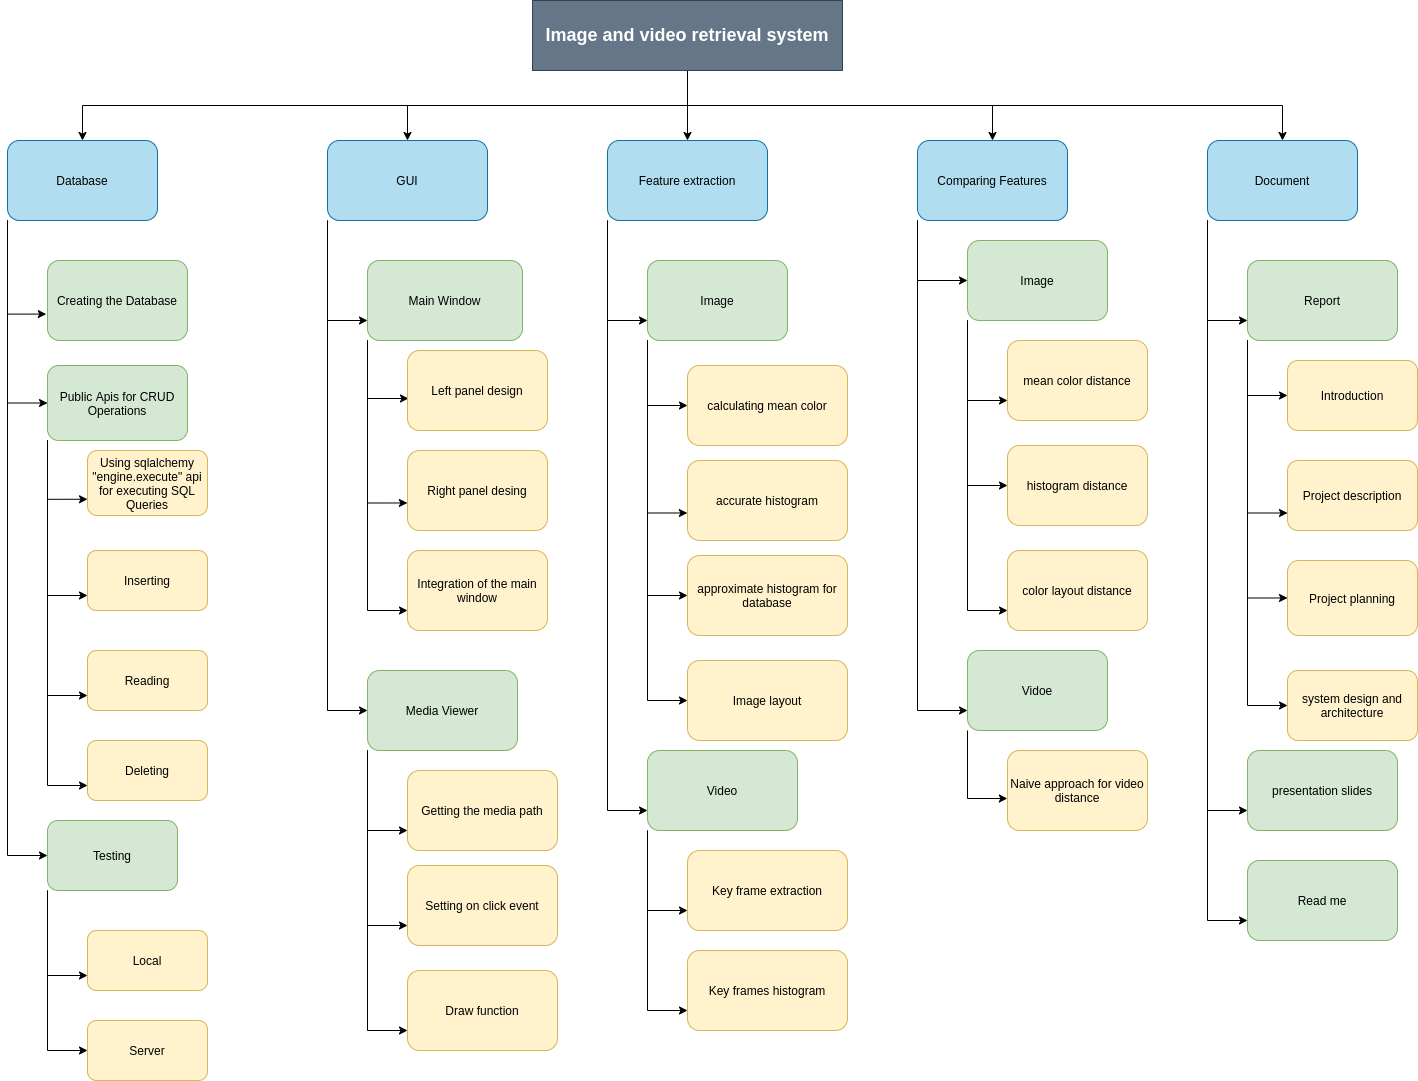
\includegraphics[width=120mm,height=100mm]{Images/TBDS.png}
    \caption{Tasks break down structure}
  \end{figure}




\section{Time plan and Gant chart}
%Begin from here

Firstly, we split all project team members into 3 basic groups in according to simplify the overall problem into 
smaller ones that we can deal with.
We decided to start with designing the database and find best modelling ways to fit our storage requirements.
The second group mission is to implement software functions that do the following:
\vskip 0.2in
\begin{enumerate}
    \item extract data from videos/images.
    \item store the different representations of input data into the database.
    \item impelemnt the required techinques that fit project targets.
\end{enumerate}
According to third group, it provides the project with a well-interactive graphical user interface.
Finally, the last group provides the project full documentation.
\vskip 0.2in
We divided our team into the following:
\begin{enumerate}
    \item Mohammed Khaled Rashad and Mohammed Hussien.
    \item Mohamed Amr Ahmed, Mohamed Amr Mohamed, Mohamed Khaled \vskip 0.05in
     Elkhawas and Mohamed Ahmed Abdel Azem.
    \item Mohammed Gamal Talaat and Mohammed Emad.
    \item Mohammed Hussien Mostafa, Mohammed Ahmed Abd el Azeem and Mohammed Emad.
\end{enumerate}


\begin{figure}[H]
  \centering
  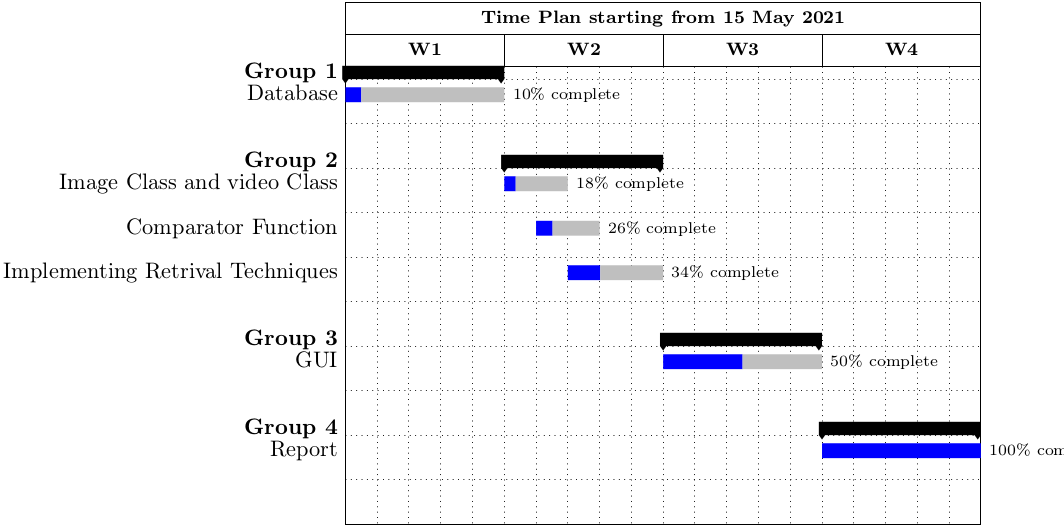
\includegraphics[width=120mm,height=90mm]{Images/time_plan.png}
  \caption{Time Plan starting from 15 May 2021}
\end{figure}
\vskip 0.2in